\chapter{Usar ramas en git}

La creación de ramas (llamadas \textbf{\textit{branches}}) en un repositorio nos permite realizar pruebas, añadir características nuevas, o cambiar de ámbito sin perjudicar el flujo de trabajo principal.

Una rama es una bifurcación del camino principal del desarrollo de una aplicación (o de un commit concreto). Esta rama puede ser una rama pública (existir en GitHub) o ser privada (sólo existir en nuestro repositorio local).

La creación de ramas en Git es instantáneo (al contrario de lo que sucedía con sistemas anteriores), por lo que crearla no supone un esfuerzo ni una pérdida de tiempo para el desarrollo.

\begin{center}
    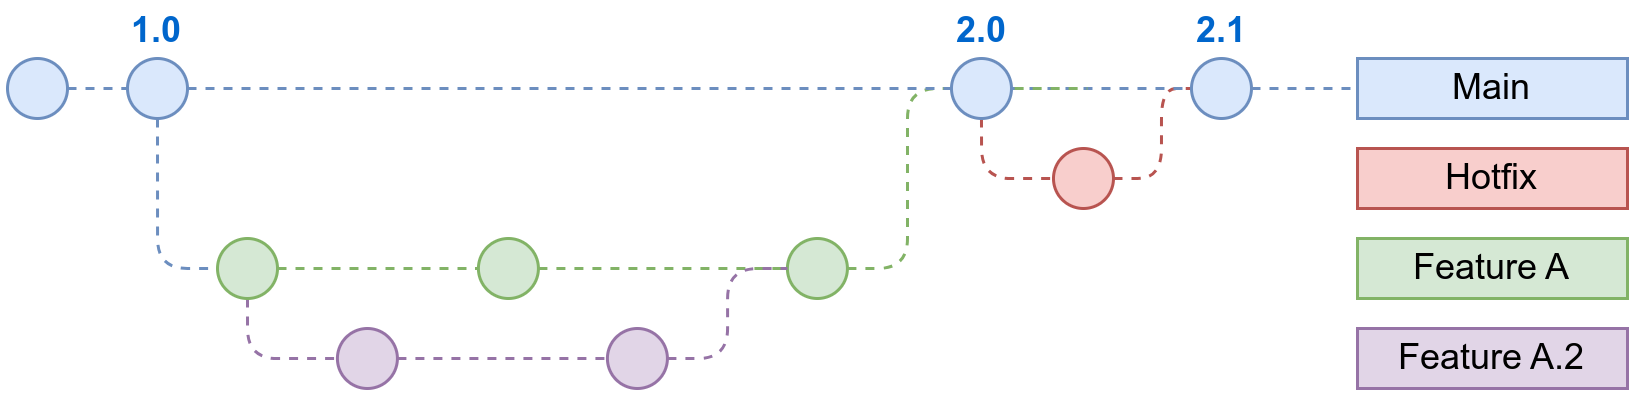
\includegraphics[width=0.9\linewidth]{ramas.png}
    \captionof{figure}{Un desarrollo con ramas}
\end{center}

En el dibujo aparecen ramas que posteriormente se unen a la rama \textit{main} principal, pero esto no tiene por qué ser así, y una rama puede mantener un desarrollo paralelo y nunca unirse.

\section{Crear rama}
Para crear una rama en el desarrollo, desde el punto en el que nos encontramos, se puede hacer de dos maneras. El resultado es el mismo, pero conviene entender qué es lo que sucede en ambos casos.

\begin{itemize}
    \item \textbf{Crear rama y luego movernos a ella}: Este caso consta de dos pasos.

\begin{mycode}{Crear rama “featureA” y movernos a ella}{console}{}
ruben@vega:~/pruebas$ git branch featureA
ruben@vega:~/pruebas$ git checkout featureA
Cambiado a rama 'feature1'

ruben@vega:~/pruebas$ git log
commit 170f9ce8c214b82f... (HEAD -> featureA, origin/main, main)
Author: Rubén Gómez <ruben@example.com>
Date:   Sun Sep 17 18:40:37 2023 +0200
...
\end{mycode}

    Tal como se puede ver, se ha creado la rama con nombre “featureA”, para posteriormente con el comando \commandbox{git checkout featureA} cambiarnos a dicha rama.

    Con \commandbox{git log} podemos comprobar cómo en ese \textit{commit} ahora mismo se encuentran tres puntos de nuestro sistema de repositorios:
    \begin{itemize}
        \item \texttt{\textbf{HEAD -> featureA}}: que es la rama en la que nos encontramos ahora.
        \item \textbf{origin/main}: la rama “main” del repositorio remoto.
        \item \textbf{main}: la rama local “main”.
    \end{itemize}

    Los tres puntos coinciden porque no se han realizado todavía ningún cambio en ninguna rama.

    \item \textbf{Crear rama y movernos a ella automáticamente}: en este caso los dos pasos se convierten en uno, pero el resultado es el mismo.

\begin{mycode}{Crear rama “featureB” y movernos a ella directamente}{console}{}
ruben@vega:~/pruebas$ git checkout -b featureB
Cambiado a nueva rama 'featureB'
\end{mycode}
\end{itemize}

\section{Cambiar entre ramas}

Ahora que ya sabemos cómo crear ramas, hay que entender cómo podemos cambiar entre ellas, aunque el comando lo acabamos de ver en el punto anterior: \commandbox{git checkout branch}, donde “branch” es el nombre de la rama a la que queremos ir.

Siguiendo con el ejemplo anterior, si queremos volver a la rama “main”, deberíamos hacer:

\begin{mycode}{Volver a la rama “main”}{console}{}
ruben@vega:~/pruebas$ git checkout main
Cambiado a rama 'main'
Tu rama está actualizada con 'origin/main'.
\end{mycode}

Si queremos volver a la rama “featureA”:

\begin{mycode}{Volver a la rama “featureA”}{console}{}
ruben@vega:~/pruebas$ git checkout featureA
Cambiado a rama 'featureA'
\end{mycode}

\section{Ver estado de las ramas}

Para comprobar cuál es el estado de las ramas, vamos a realizar dos \textit{commits} distintos en la rama “main” y otro en la rama “featureA”. Para ver cómo se encuentra ahora el estado de nuestro repositorio, podemos hacer uso del siguiente comando:

\begin{mycode}{Volver a la rama “featureA”}{console}{{\footnotesize }}
$ git log --graph --all --pretty=format:'%Cred%h%Creset -%C(auto)%d%Creset %s  %Creset'
\end{mycode}

Obtendríamos el siguiente resultado:

\begin{center}
    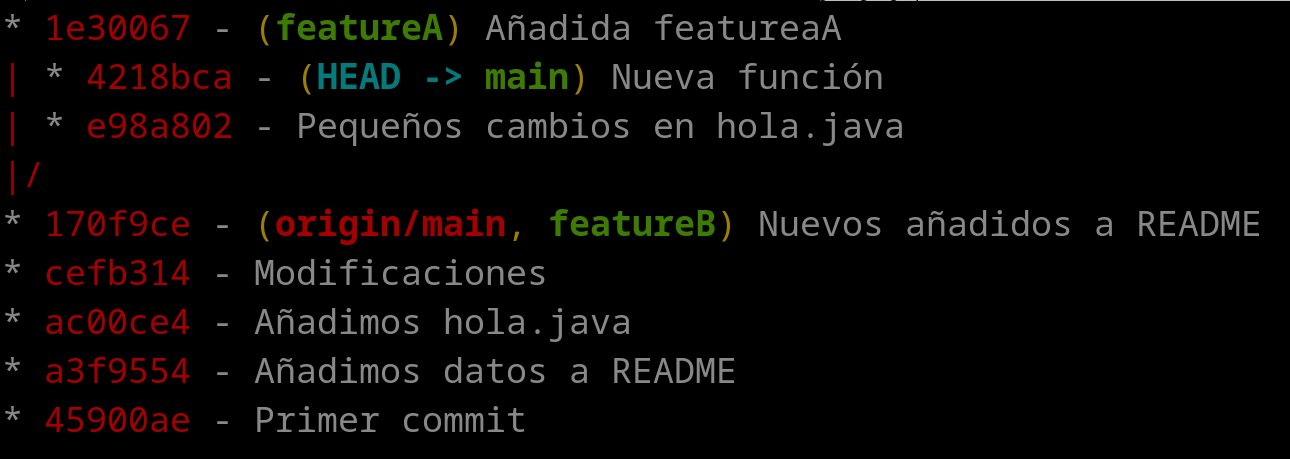
\includegraphics[width=0.9\linewidth]{ramas2.png}
    \captionof{figure}{Ramas actuales}
\end{center}

Tal como se puede ver, la bifurcación sucede en el commit “170f9ce”, que es donde está situado el último commit del servidor remoto y la rama “featureB” creada previamente (y que no se ha tocado).

Por otro lado, desde ese punto surgen dos ramas:
\begin{itemize}
    \item \textbf{featureA}, con el único commit 1e30067.
    \item \textbf{main}, que tiene 2 commits.
\end{itemize}

Tras realizar estas modificaciones, a continuación vamos a ver cómo podemos fusionar los cambios de una rama en la otra.


\chapter{Fusionar ramas}

La fusión de ramas (en inglés \textit{\textbf{merge}}) sucede cuando queremos obtener los cambios realizados en una rama y fusionar dichos cambios con la rama en la que nos encontramos actualmente.  Ahora que tenemos distintas ramas creadas, con sus correspondientes commits, es buen momento para realizar la fusión de las ramas.

Dependiendo de cómo haya sido el desarrollo de las ramas, la fusión podrá terminar en un “dibujo” distinto. Por ejemplo, el caso más sencillo es que en la bifurcación sólo la rama nueva tiene nuevos commits, por lo que al realizar la fusión quedaría:


\begin{center}
    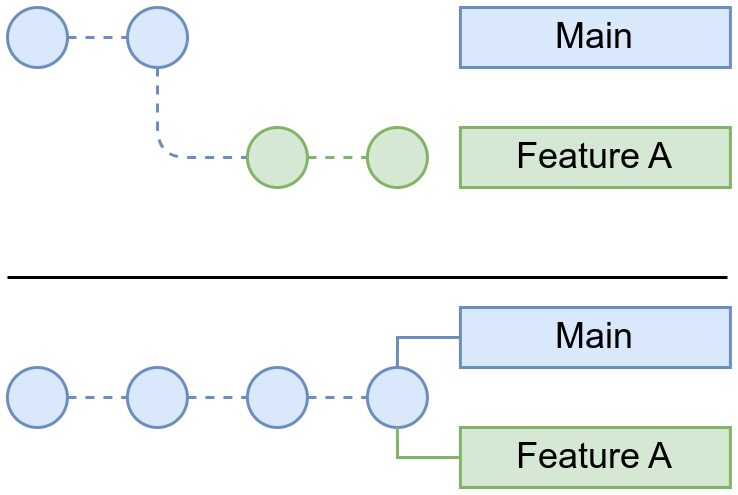
\includegraphics[width=0.6\linewidth]{merge_facil.png}
    \captionof{figure}{Merge de rama con commits sobre rama “main”}
\end{center}

Tras realizar el merge, en este caso es como si la rama “FeatureA”no hubiese existido.

En cambio, si en la rama main, tal como se ha sugerido en el punto anterior, también se realizan modificaciones, el dibujo quedará tal que así:

\begin{center}
    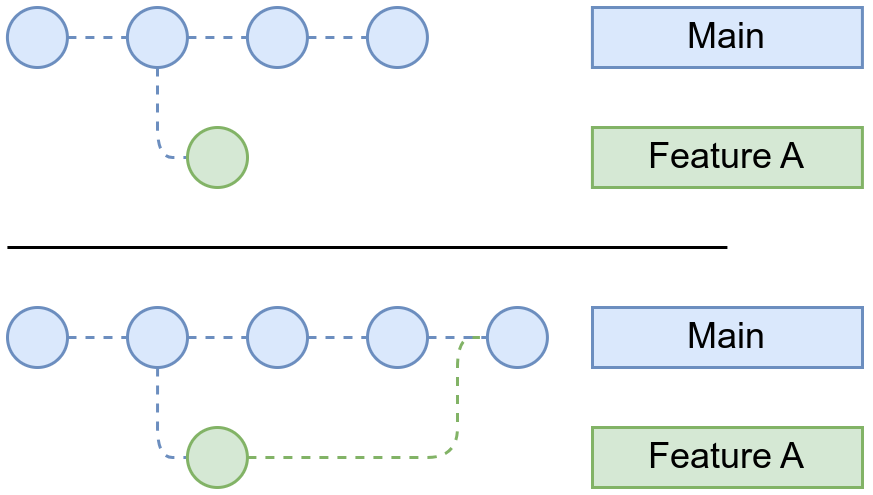
\includegraphics[width=0.6\linewidth]{merge_serio.png}
    \captionof{figure}{Merge donde hay commits en ambas ramas}
\end{center}


Para realizar la fusión, debemos seguir estos pasos:
\begin{itemize}
    \item Colocarnos en la rama en la que queremos fusionar los cambios de otra rama. Normalmente, nos va a interesar añadir los cambios a la rama “main”.
    \item Realizar la fusión.
\end{itemize}


\begin{mycode}{Volver a la rama “main”}{console}{}
ruben@vega:~/pruebas$ git checkout main
ruben@vega:~/pruebas$ git merge featureA -m "Merge de FeatureA en main"
\end{mycode}

De esta manera, crearemos un nuevo commit con el texto “Merge de FeatureA en main”, que indicará la fusión de la rama “featureA” sobre la rama Main. El dibujo en la vida real queda de la siguiente manera:


\begin{center}
    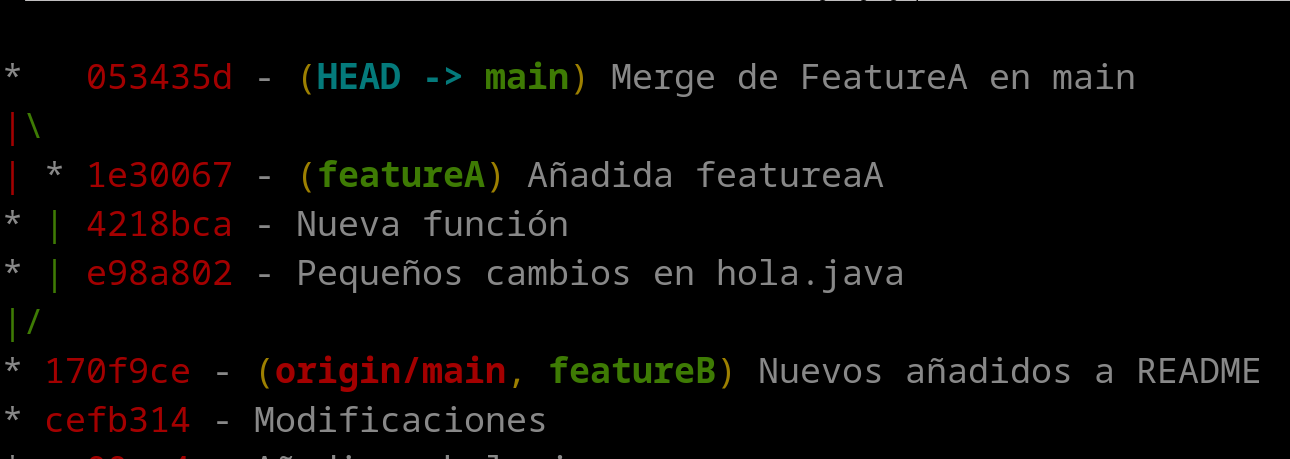
\includegraphics[width=0.9\linewidth]{merge_final.png}
    \captionof{figure}{Merge donde hay commits en ambas ramas}
\end{center}

Una vez realizado el \textit{merge}, podemos subir los cambios al repositorio central. La rama “featuresA” es una rama local, por lo que a nivel de GitHub esa rama nunca ha existido, aunque podemos ver en el interfaz web que el gráfico sí ha sufrido una ramificación:

\begin{center}
    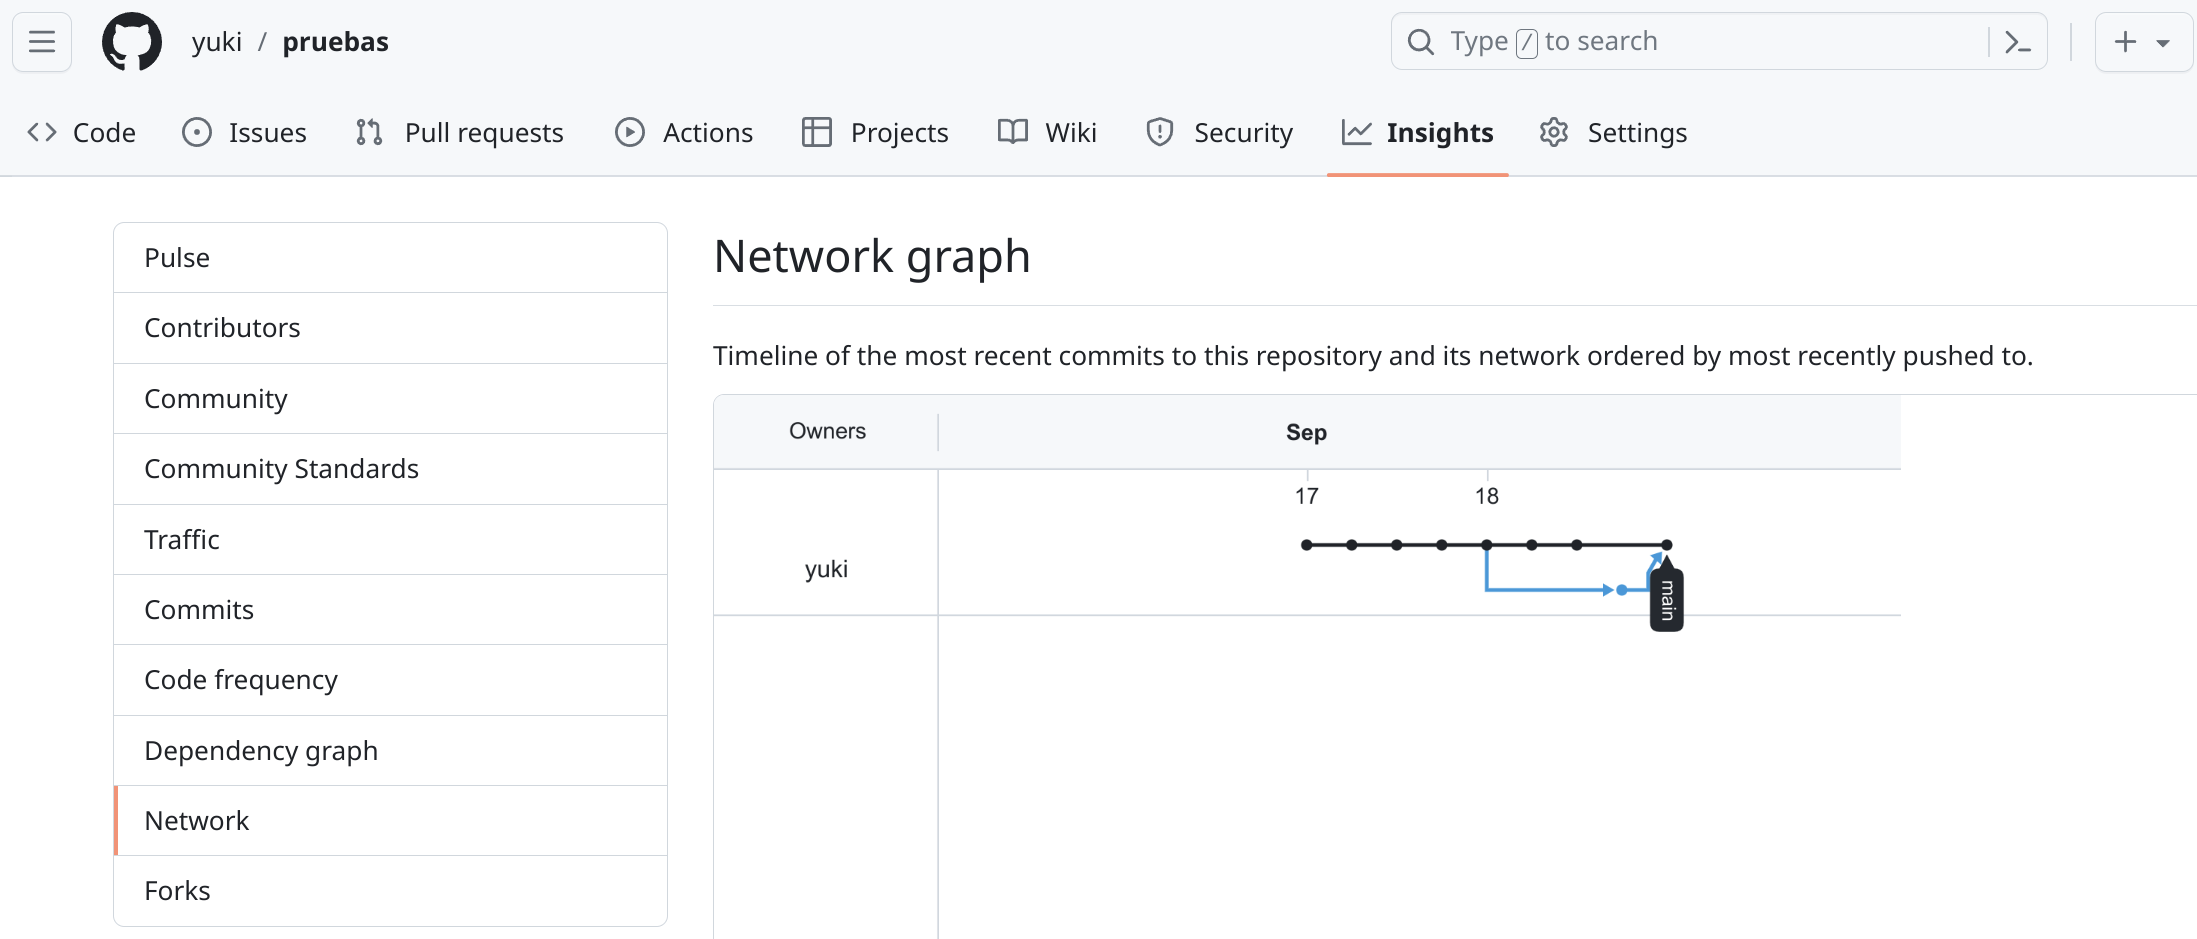
\includegraphics[frame,width=0.9\linewidth]{merge_github.png}
    \captionof{figure}{Gráfico en el interfaz de GitHub}
\end{center}